\documentclass[classical]{einfart}
\usepackage{ProjLib}
\usepackage{hologo}
\usepackage{graphicx} %插入图片的宏包
\usepackage{float} %设置图片浮动位置的宏包
\usepackage{subfigure} %插入多图时用子图显示的宏包
\usepackage{hyperref}

\UseLanguage{TC}
%%================================
%% Titles
%%================================
\let\LevelOneTitle\section
\let\LevelTwoTitle\subsection
\let\LevelThreeTitle\subsubsection

\providecommand{\tightlist}{%
  \setlength{\itemsep}{0pt}\setlength{\parskip}{0pt}}

\begin{document}

\setcounter{tocdepth}{2}
{\setstretch{1.07}\tableofcontents}

\newpage

\part{個人能力}

\section{技能}

程式語言:Java、C、C++、Python、JavaScript、Shell
Script、HTML/CSS、LaTeX、SQL、Golang、Rust、Lisp

框架:Vue.js、Spring Boot、gin、OpenCV、Qt

開發平台:Arch Linux

語言:繁體中文(母語)、簡體中文(閱讀、用詞轉換)、英文(優良,目前在準備托福考試)

其他能力:能用 Figma 進行簡單原型設計、Arch Linux 打包腳本 PKGBUILD
編寫、Docker 使用 

Github: \url{https://github.com/junyussh}

個人網站:\url{https://junyussh.github.io}

\section{榮譽與獎學金}

大學期間獎狀證明均已上傳至系統,這邊不再放置。

\begin{itemize}
\tightlist
\item
  2019 台湾、港澳及华侨学生奖学金\ 二等奖
\item
  2019 全国大学生软件创新大赛\ 校級一等獎
\item
  2020 ``中国外运杯''第七届全国大学生物流设计大赛\ 校級一等獎
\item
  2021 ``中国外运杯''第七届全国大学生物流设计大赛\ 國家級優勝獎
\end{itemize}

\section{其他興趣}

\begin{itemize}
\item
  煮飯\\
  高二時由於家人去大陸工作,我一個人在台灣生活,學會了做飯的技巧,可以自給自足。去年疫情過年時因為隔離政策沒回台灣,也做飯給一同滯留在大陸的同學吃。
\item
  唱歌\\
  閒暇時喜歡聽搖滾音樂,也因為高中有加入音樂性社團,自己有練習唱歌,曾在學生組織的晚會上表演過。
\end{itemize}


\newpage
\part{活動參與}

\section{社群活動參與}

\subsection{高中}

\subsubsection*{2016}

\begin{itemize}
\tightlist
\item
  Hackathon Taiwan Junior
\item
  HP Codewars
\end{itemize}

\begin{figure}[H]
    \centering
    \subfigure[Hackathon Taiwan Junior]{\label{Fig.sub.1}
    \includegraphics[width=0.45\textwidth]{images/黑客松證明.jpeg}}
    \subfigure[HP Codewars]{\label{Fig.sub.1}
    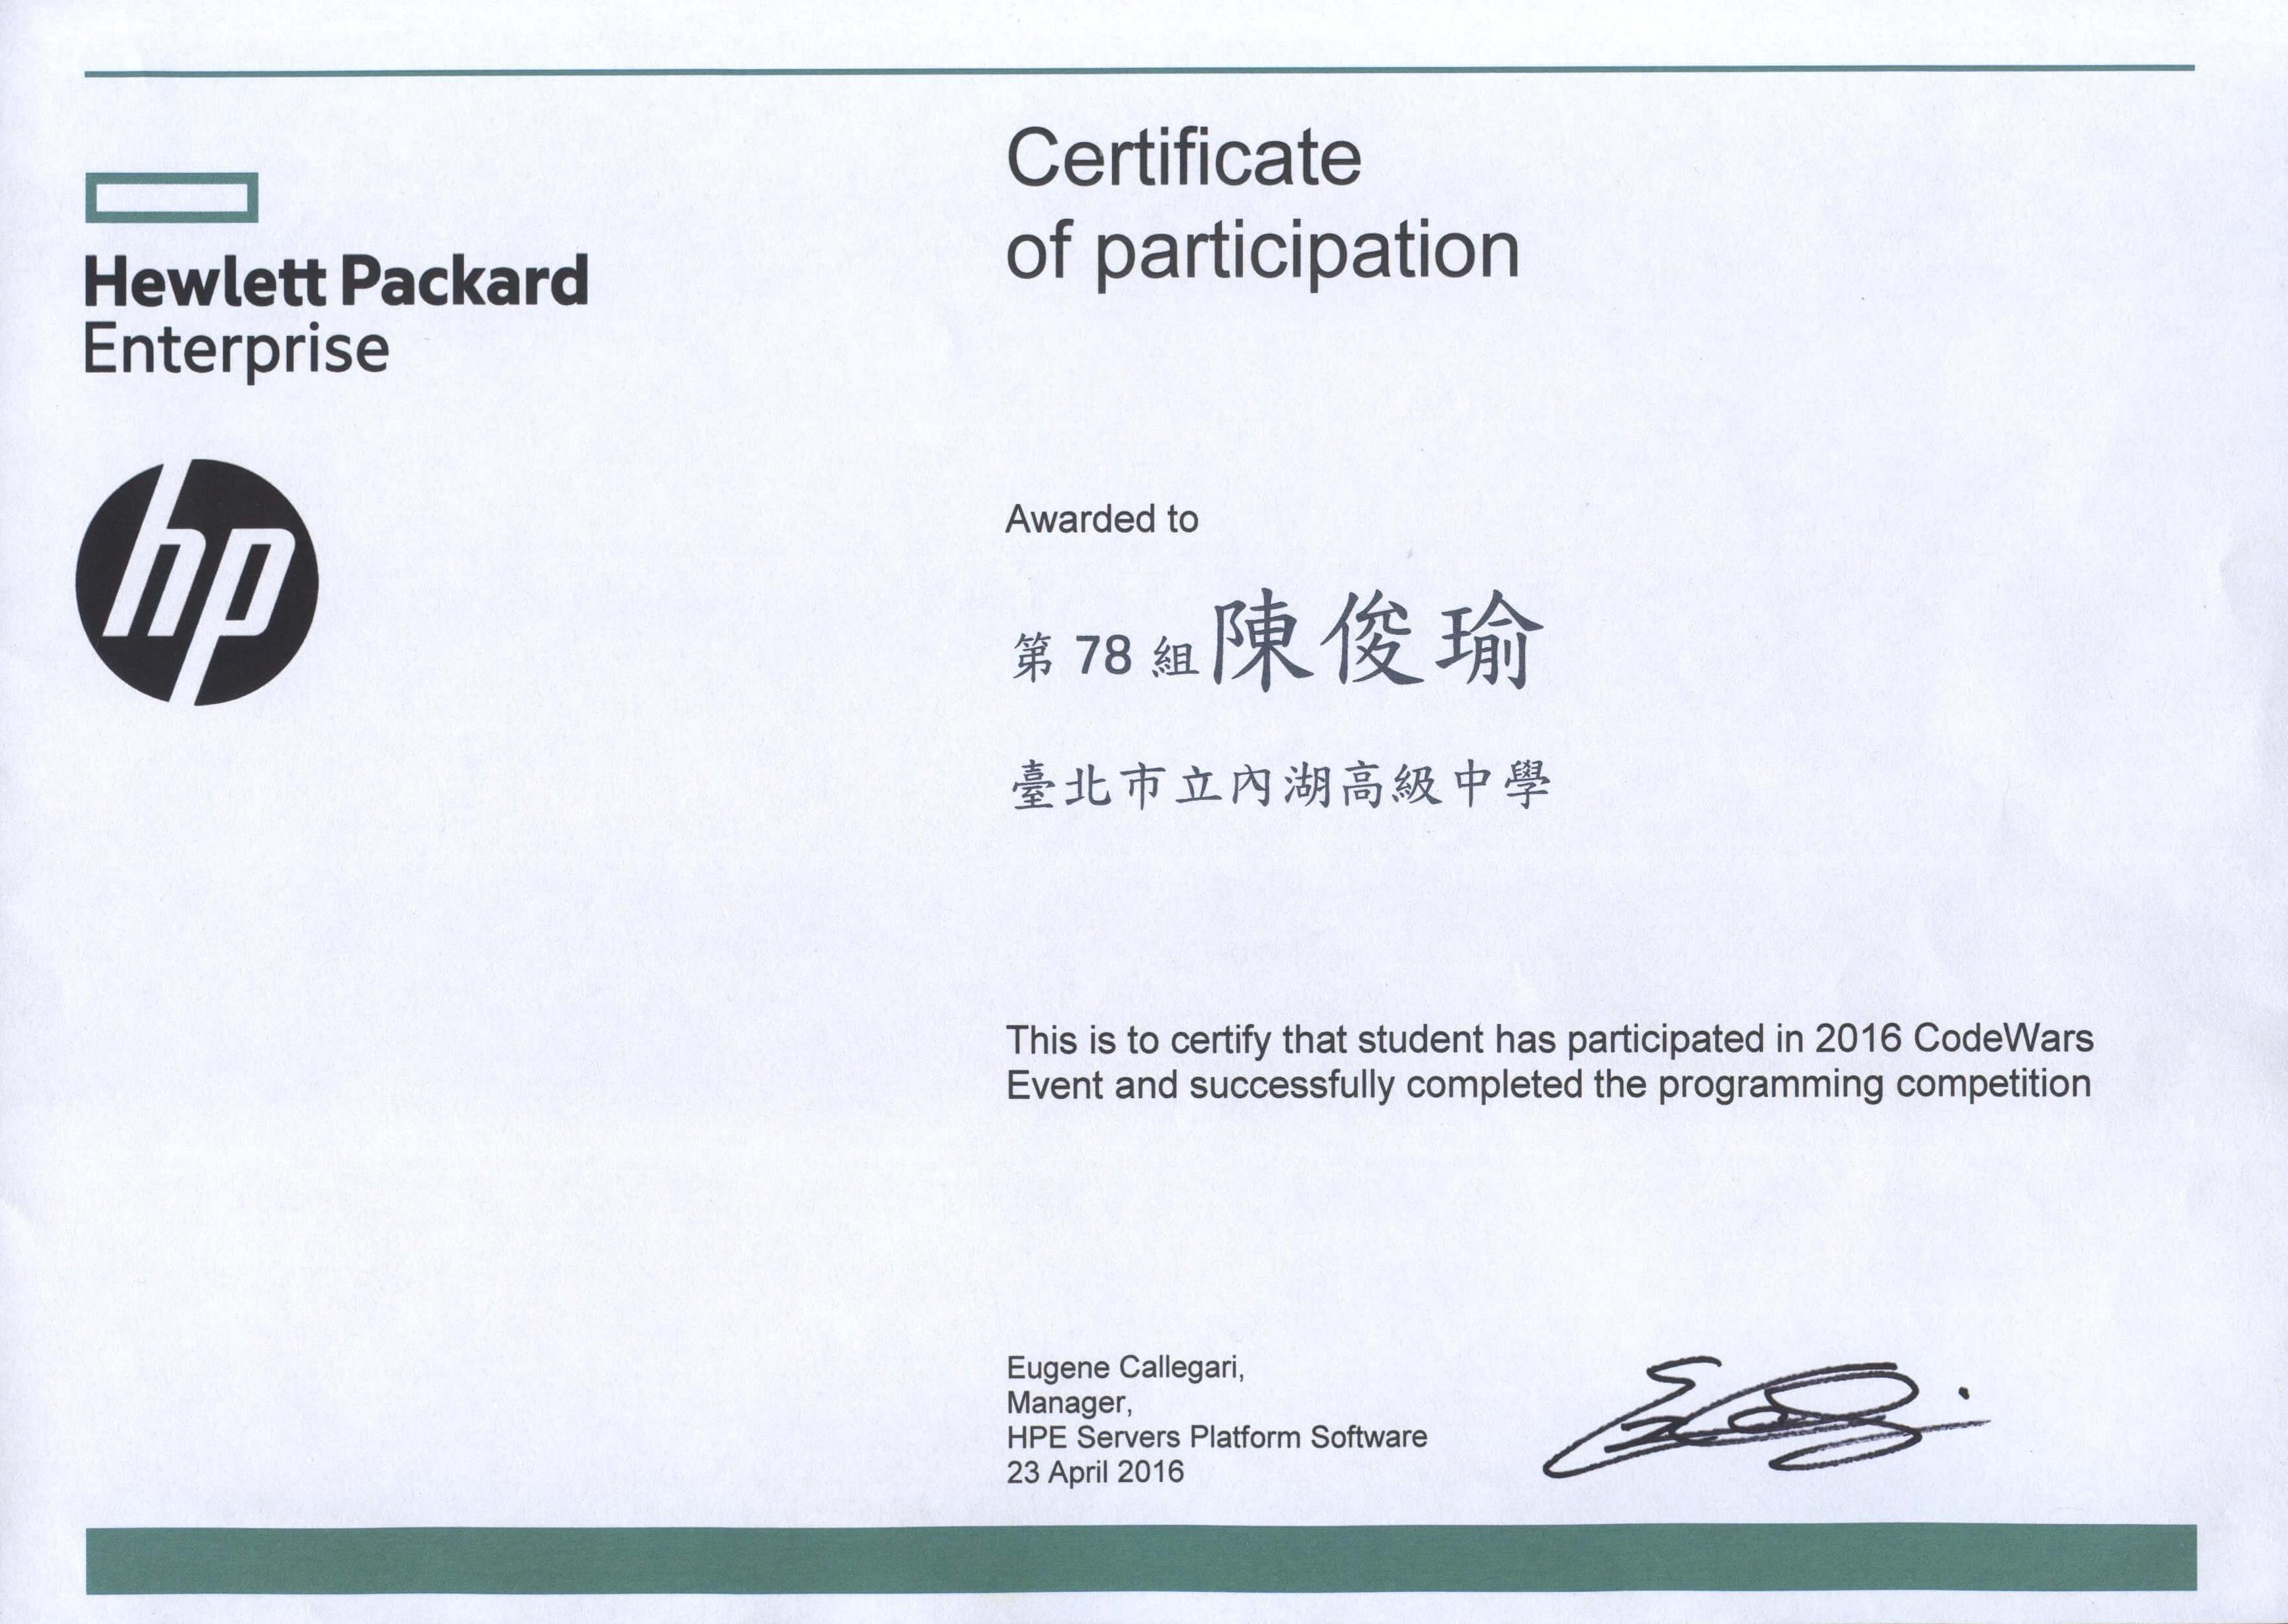
\includegraphics[width=0.45\textwidth]{images/2016 HP Codewars.jpeg}}
    \caption{證書}
\end{figure}

\subsubsection*{2017}

\begin{itemize}
\tightlist
\item
  高中資訊學術聯展---INFAS.js(攤位工作人員)
\item
  HP Codewars
\end{itemize}

\begin{figure}[H]
    \centering
    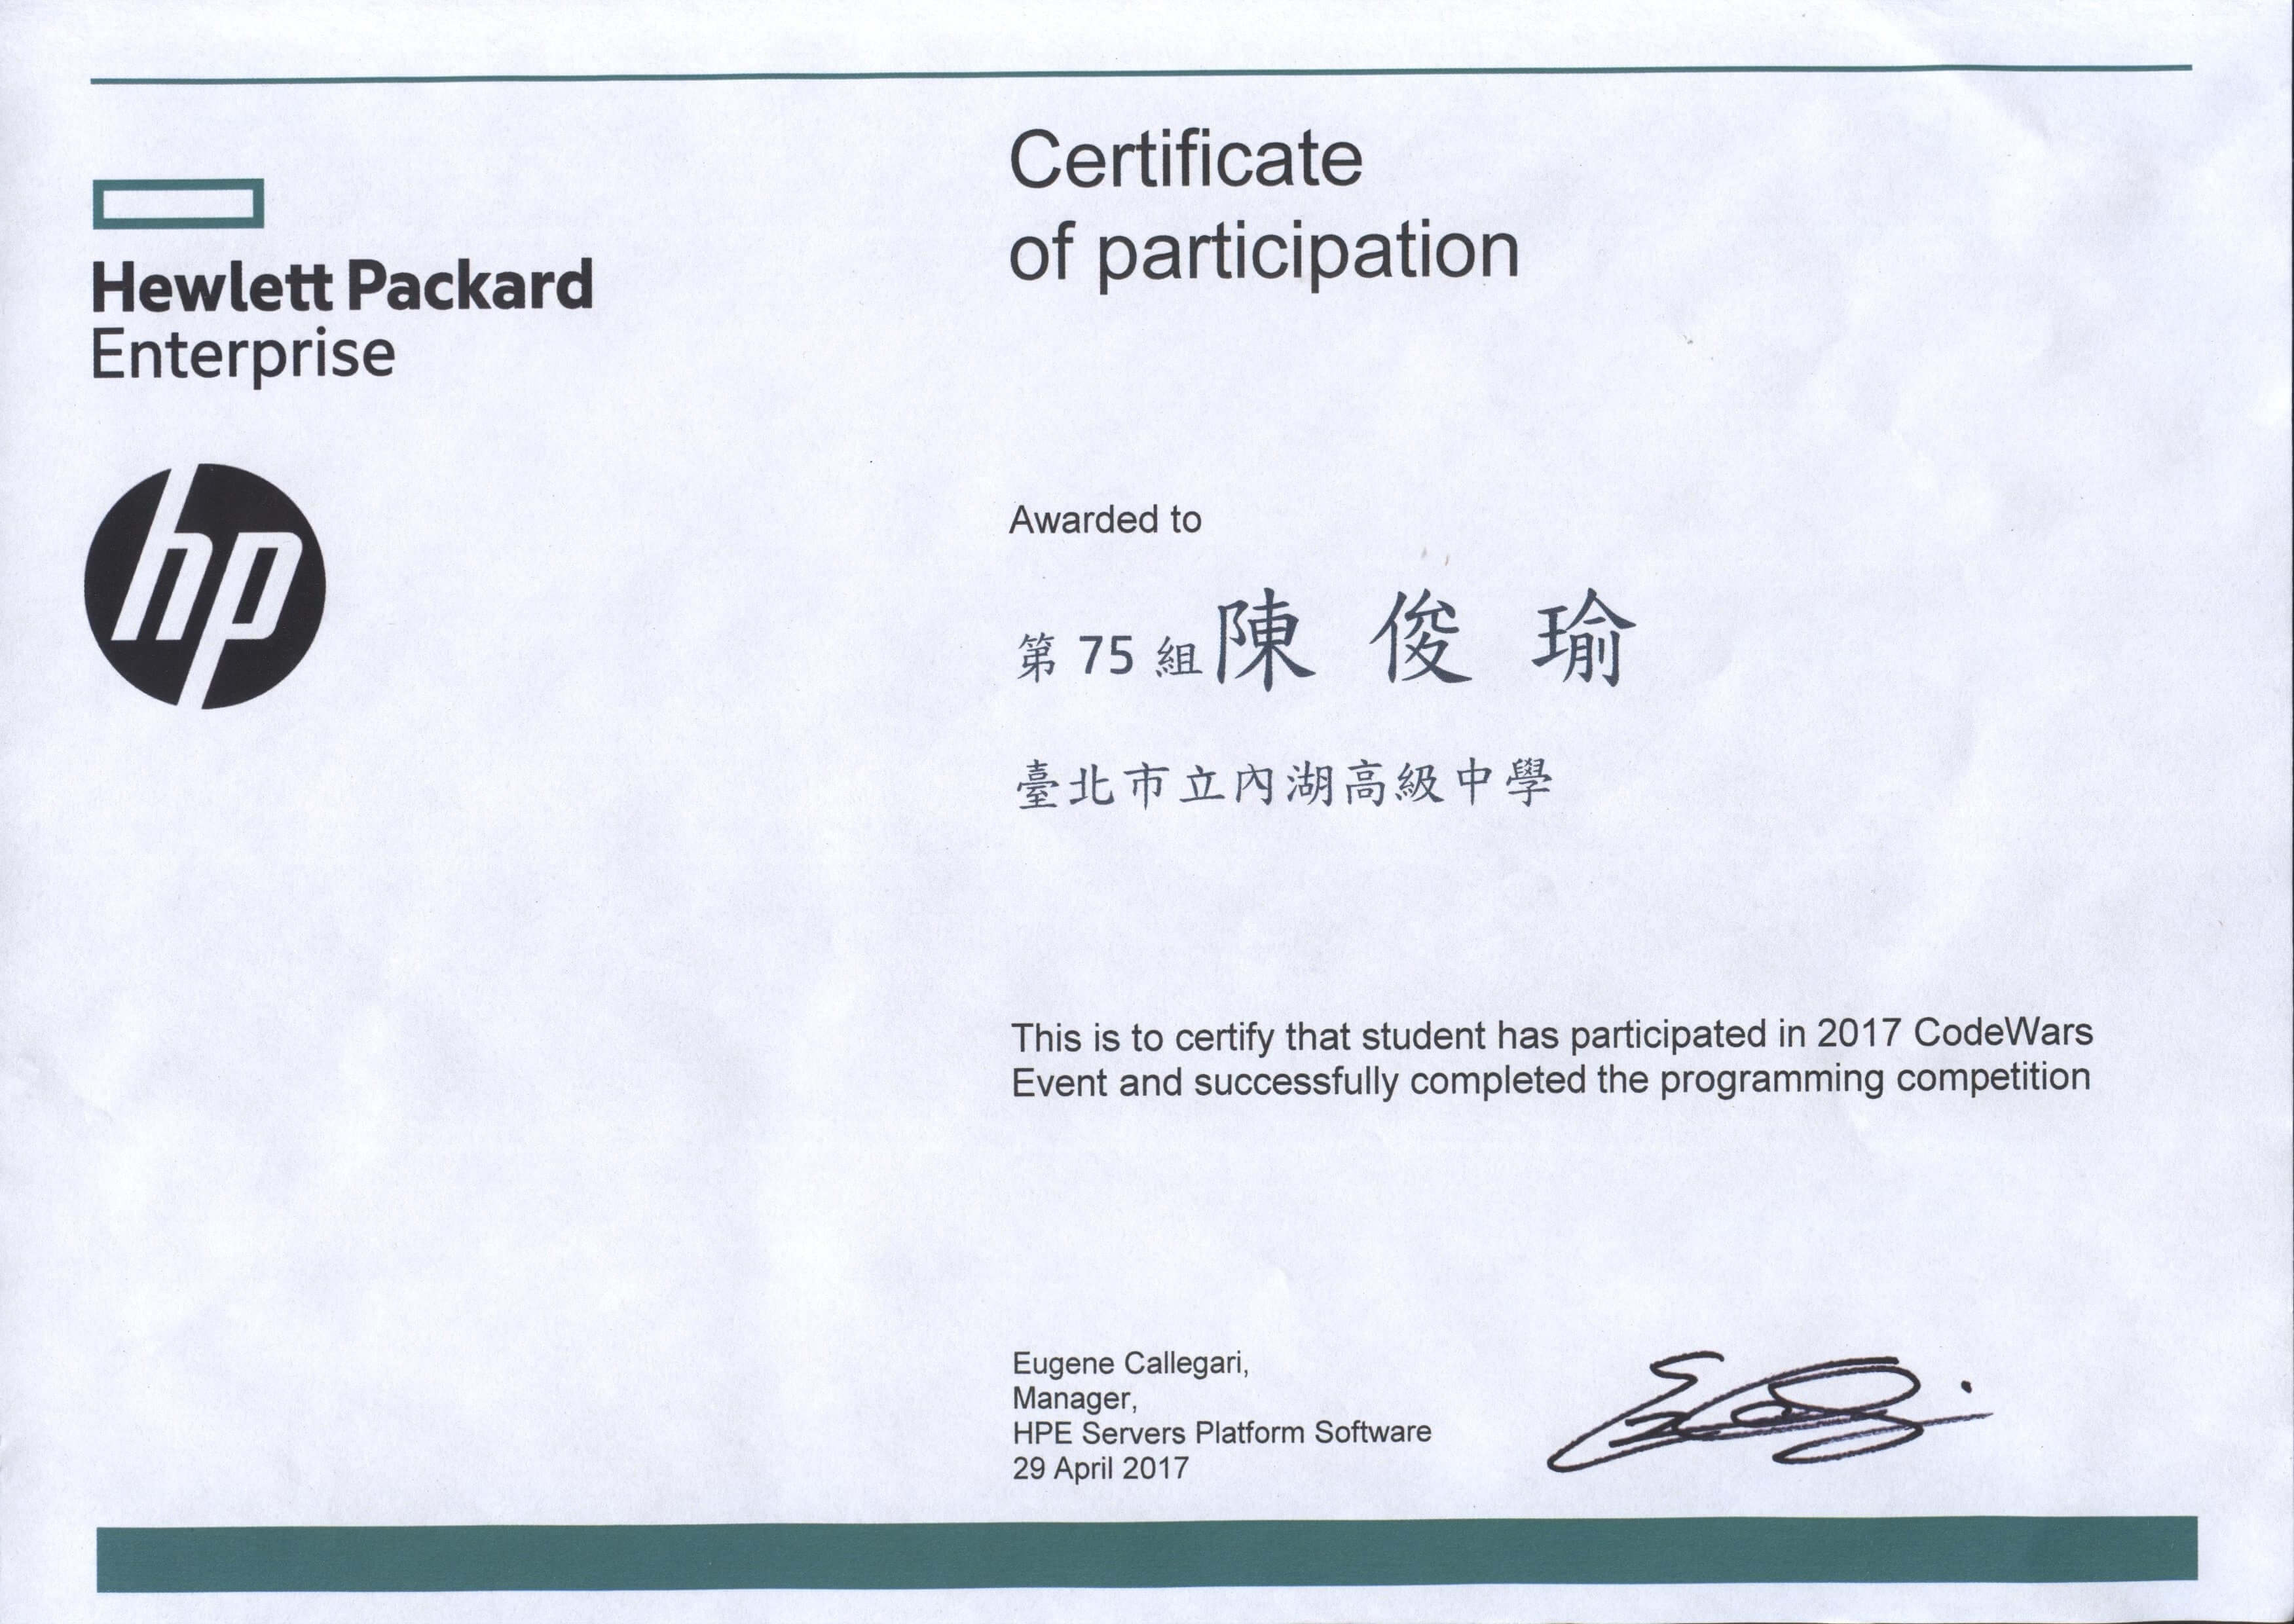
\includegraphics[width=0.7\textwidth]{images/2017 HP Codewars.jpg}
    \caption{HP Codewars 證書}
\end{figure}
% \begin{figure}[H]
%     \centering
%     \subfigure[INFAS 掛牌]{\label{Fig.sub.1}
%     \includegraphics[width=0.3\textwidth]{images/INFAS 掛牌.jpg}}
%     \subfigure[HP Codewars]{\label{Fig.sub.1}
%     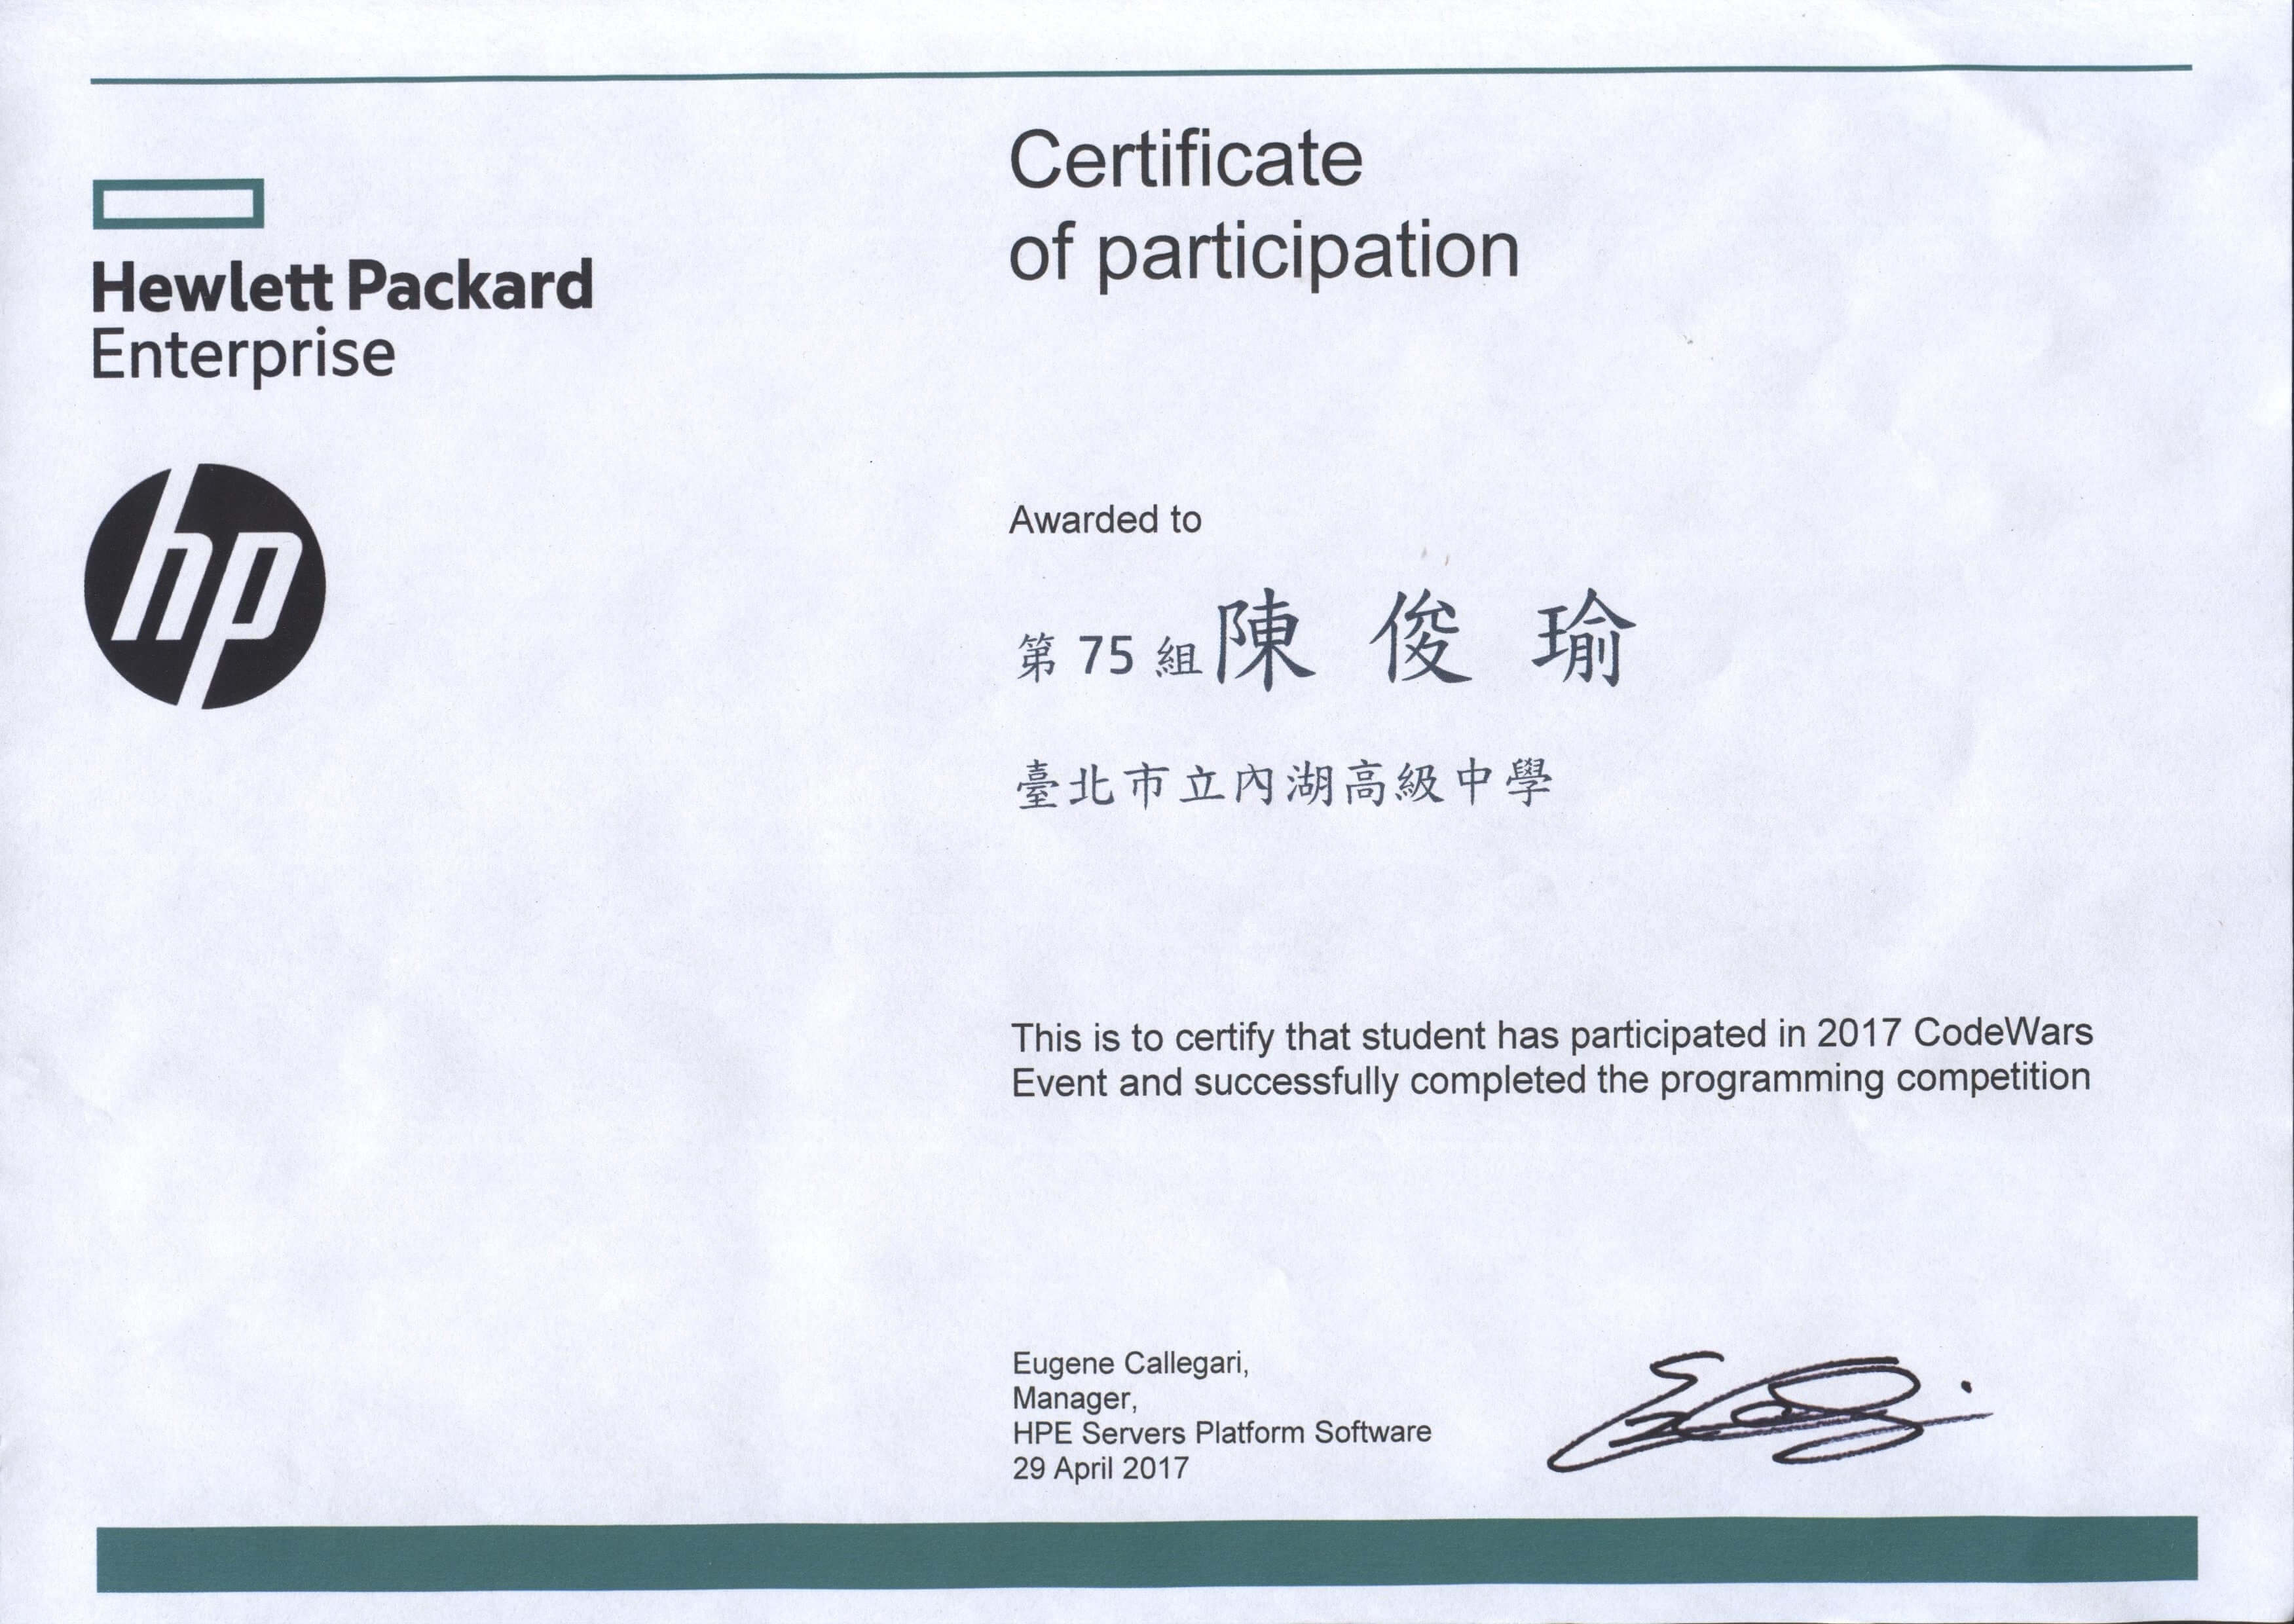
\includegraphics[width=0.6\textwidth]{images/2017 HP Codewars.jpg}
%     \caption{證書}
% \end{figure}

\subsubsection*{2018}

\begin{itemize}
\tightlist
\item
  高中資訊學術聯展---INFAS.js
\item
  國網中心資安研討會
\item
  SITCON 學生計算機年會
\item
  Google Cloud OnBoard
\item
  Microsoft Insider Dev Tour
\item
  LASS 使用者與開發者大會
\end{itemize}

\begin{figure}[H]
    \centering
    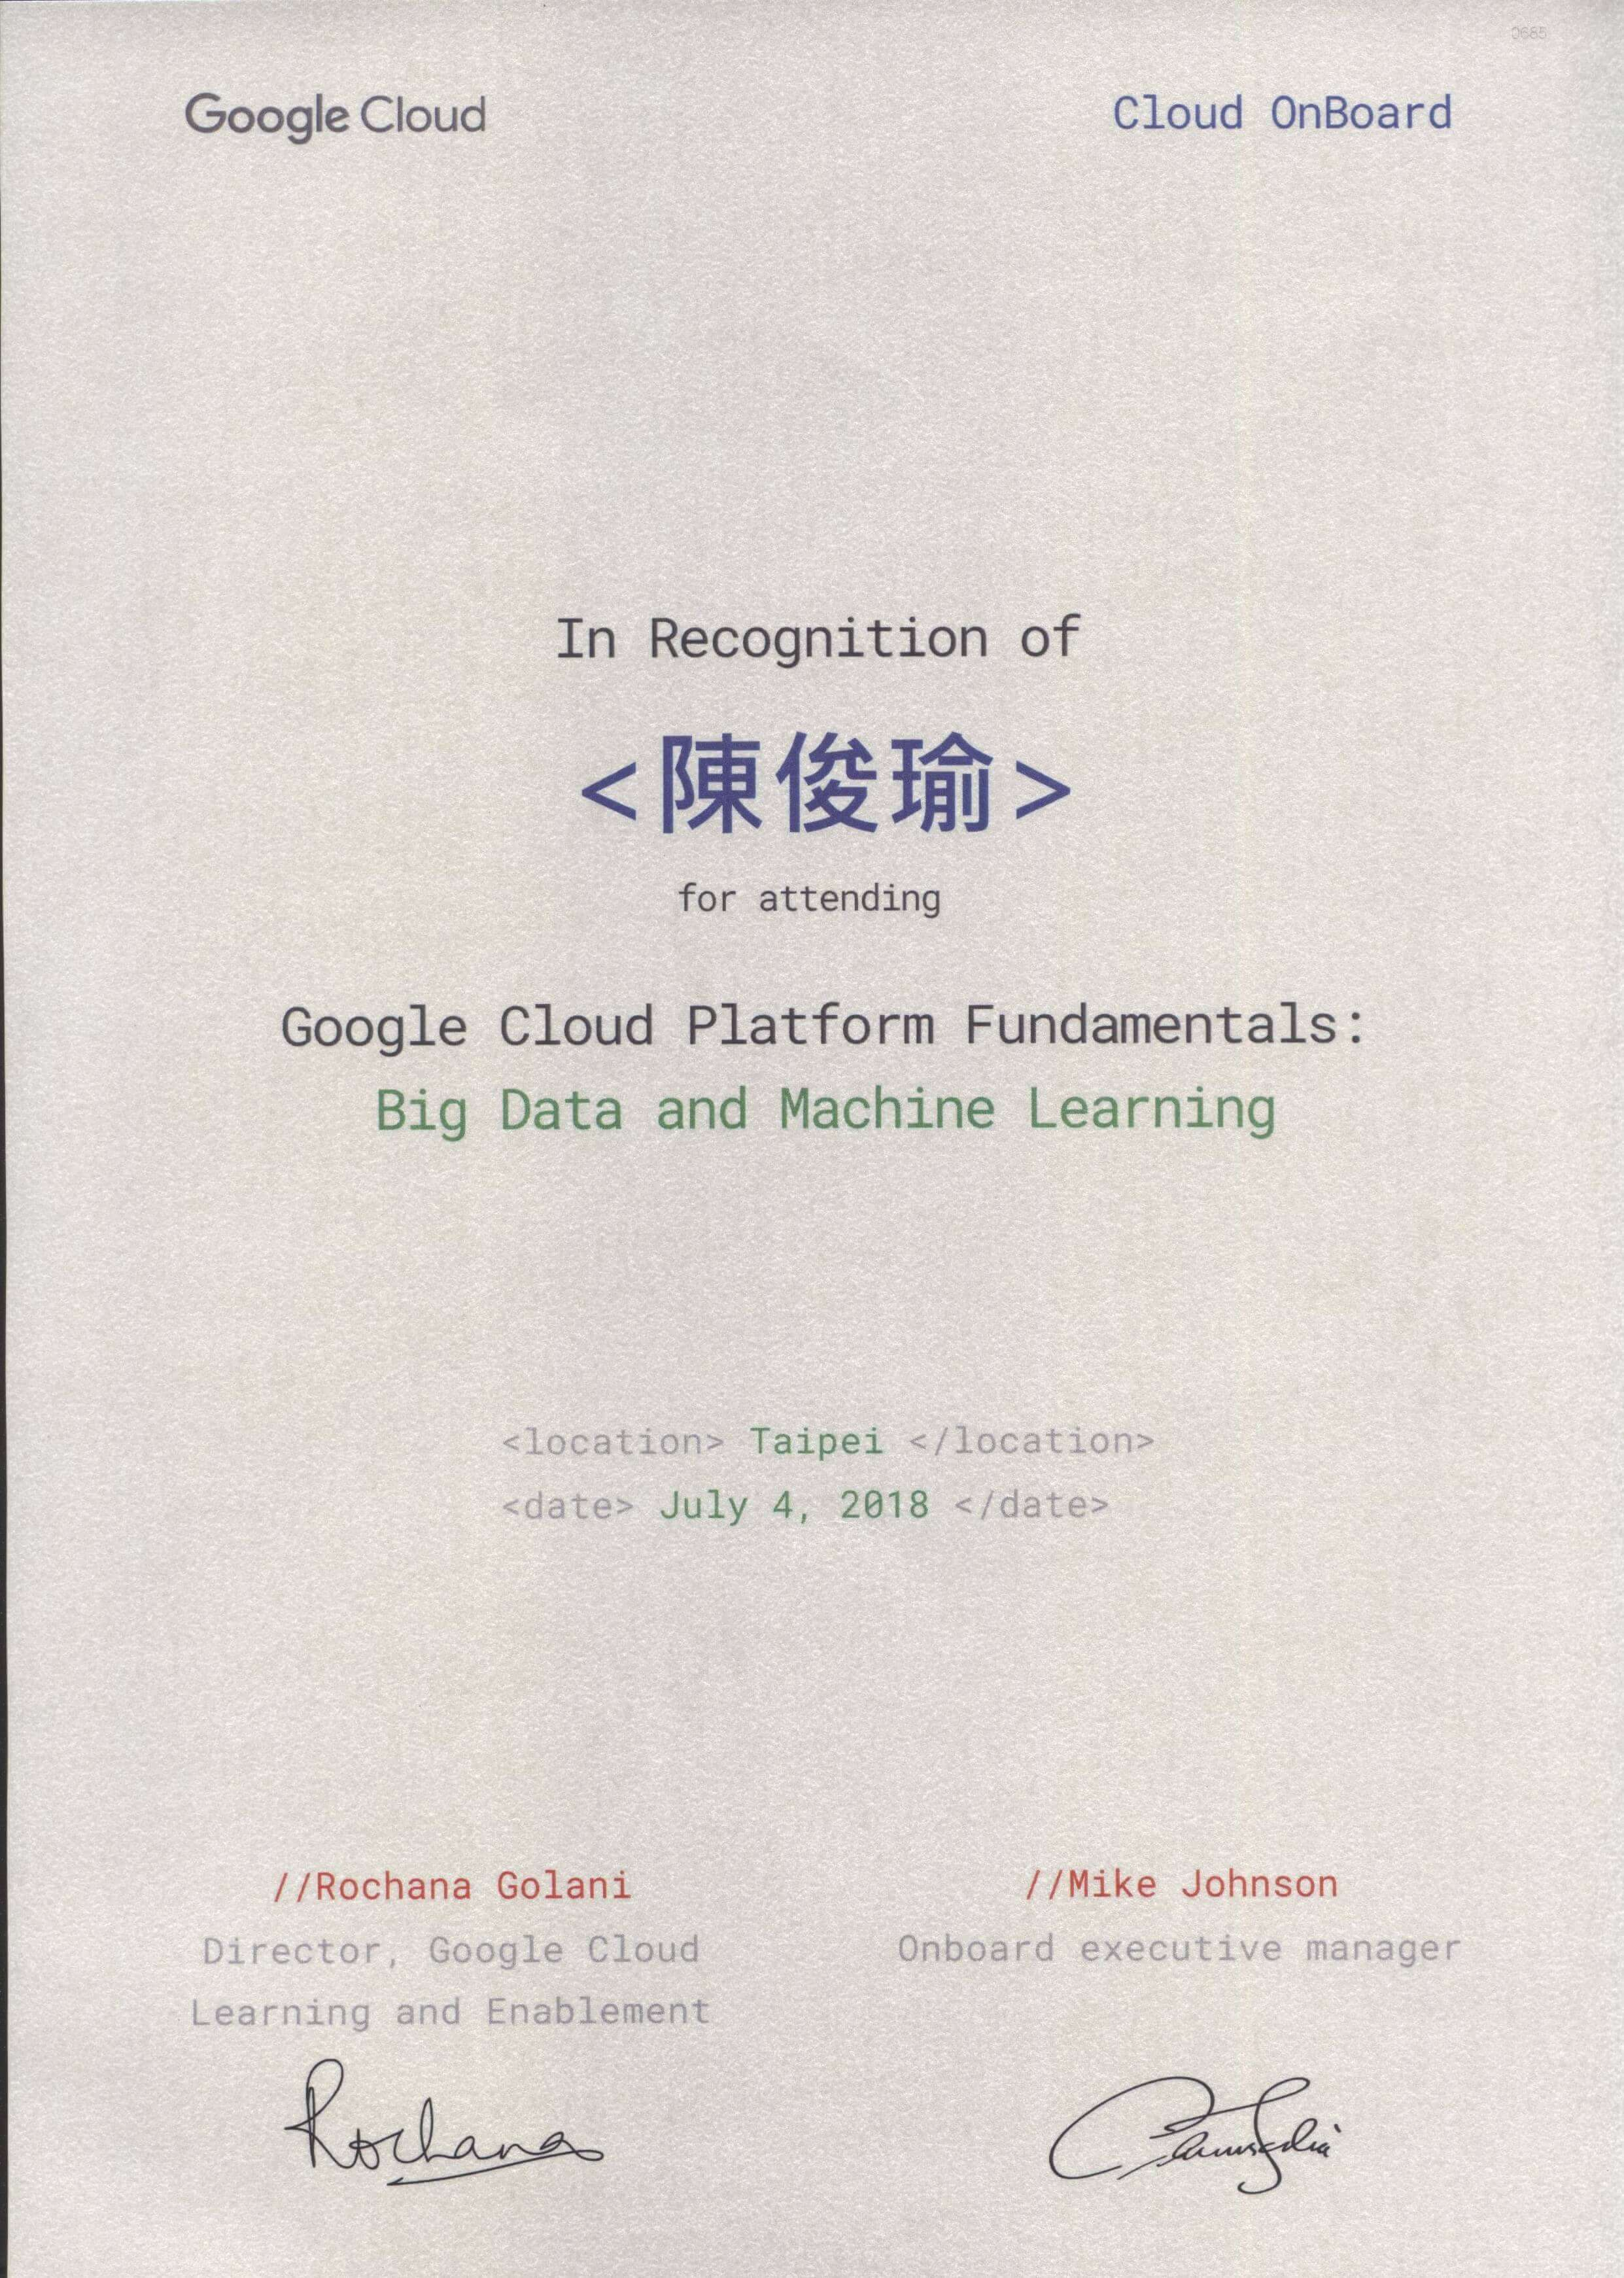
\includegraphics[height=0.6\textwidth]{images/Google Cloud OnBoard.jpg}
    \caption{Google Cloud OnBoard 證書}
\end{figure}
% \begin{figure}[H]
%     \centering
%     \subfigure[INFAS 掛牌]{\label{Fig.sub.1}
%     \includegraphics[width=0.5\textwidth]{images/SITCON 掛牌.jpg}}
%     \subfigure[HP Codewars]{\label{Fig.sub.1}
%     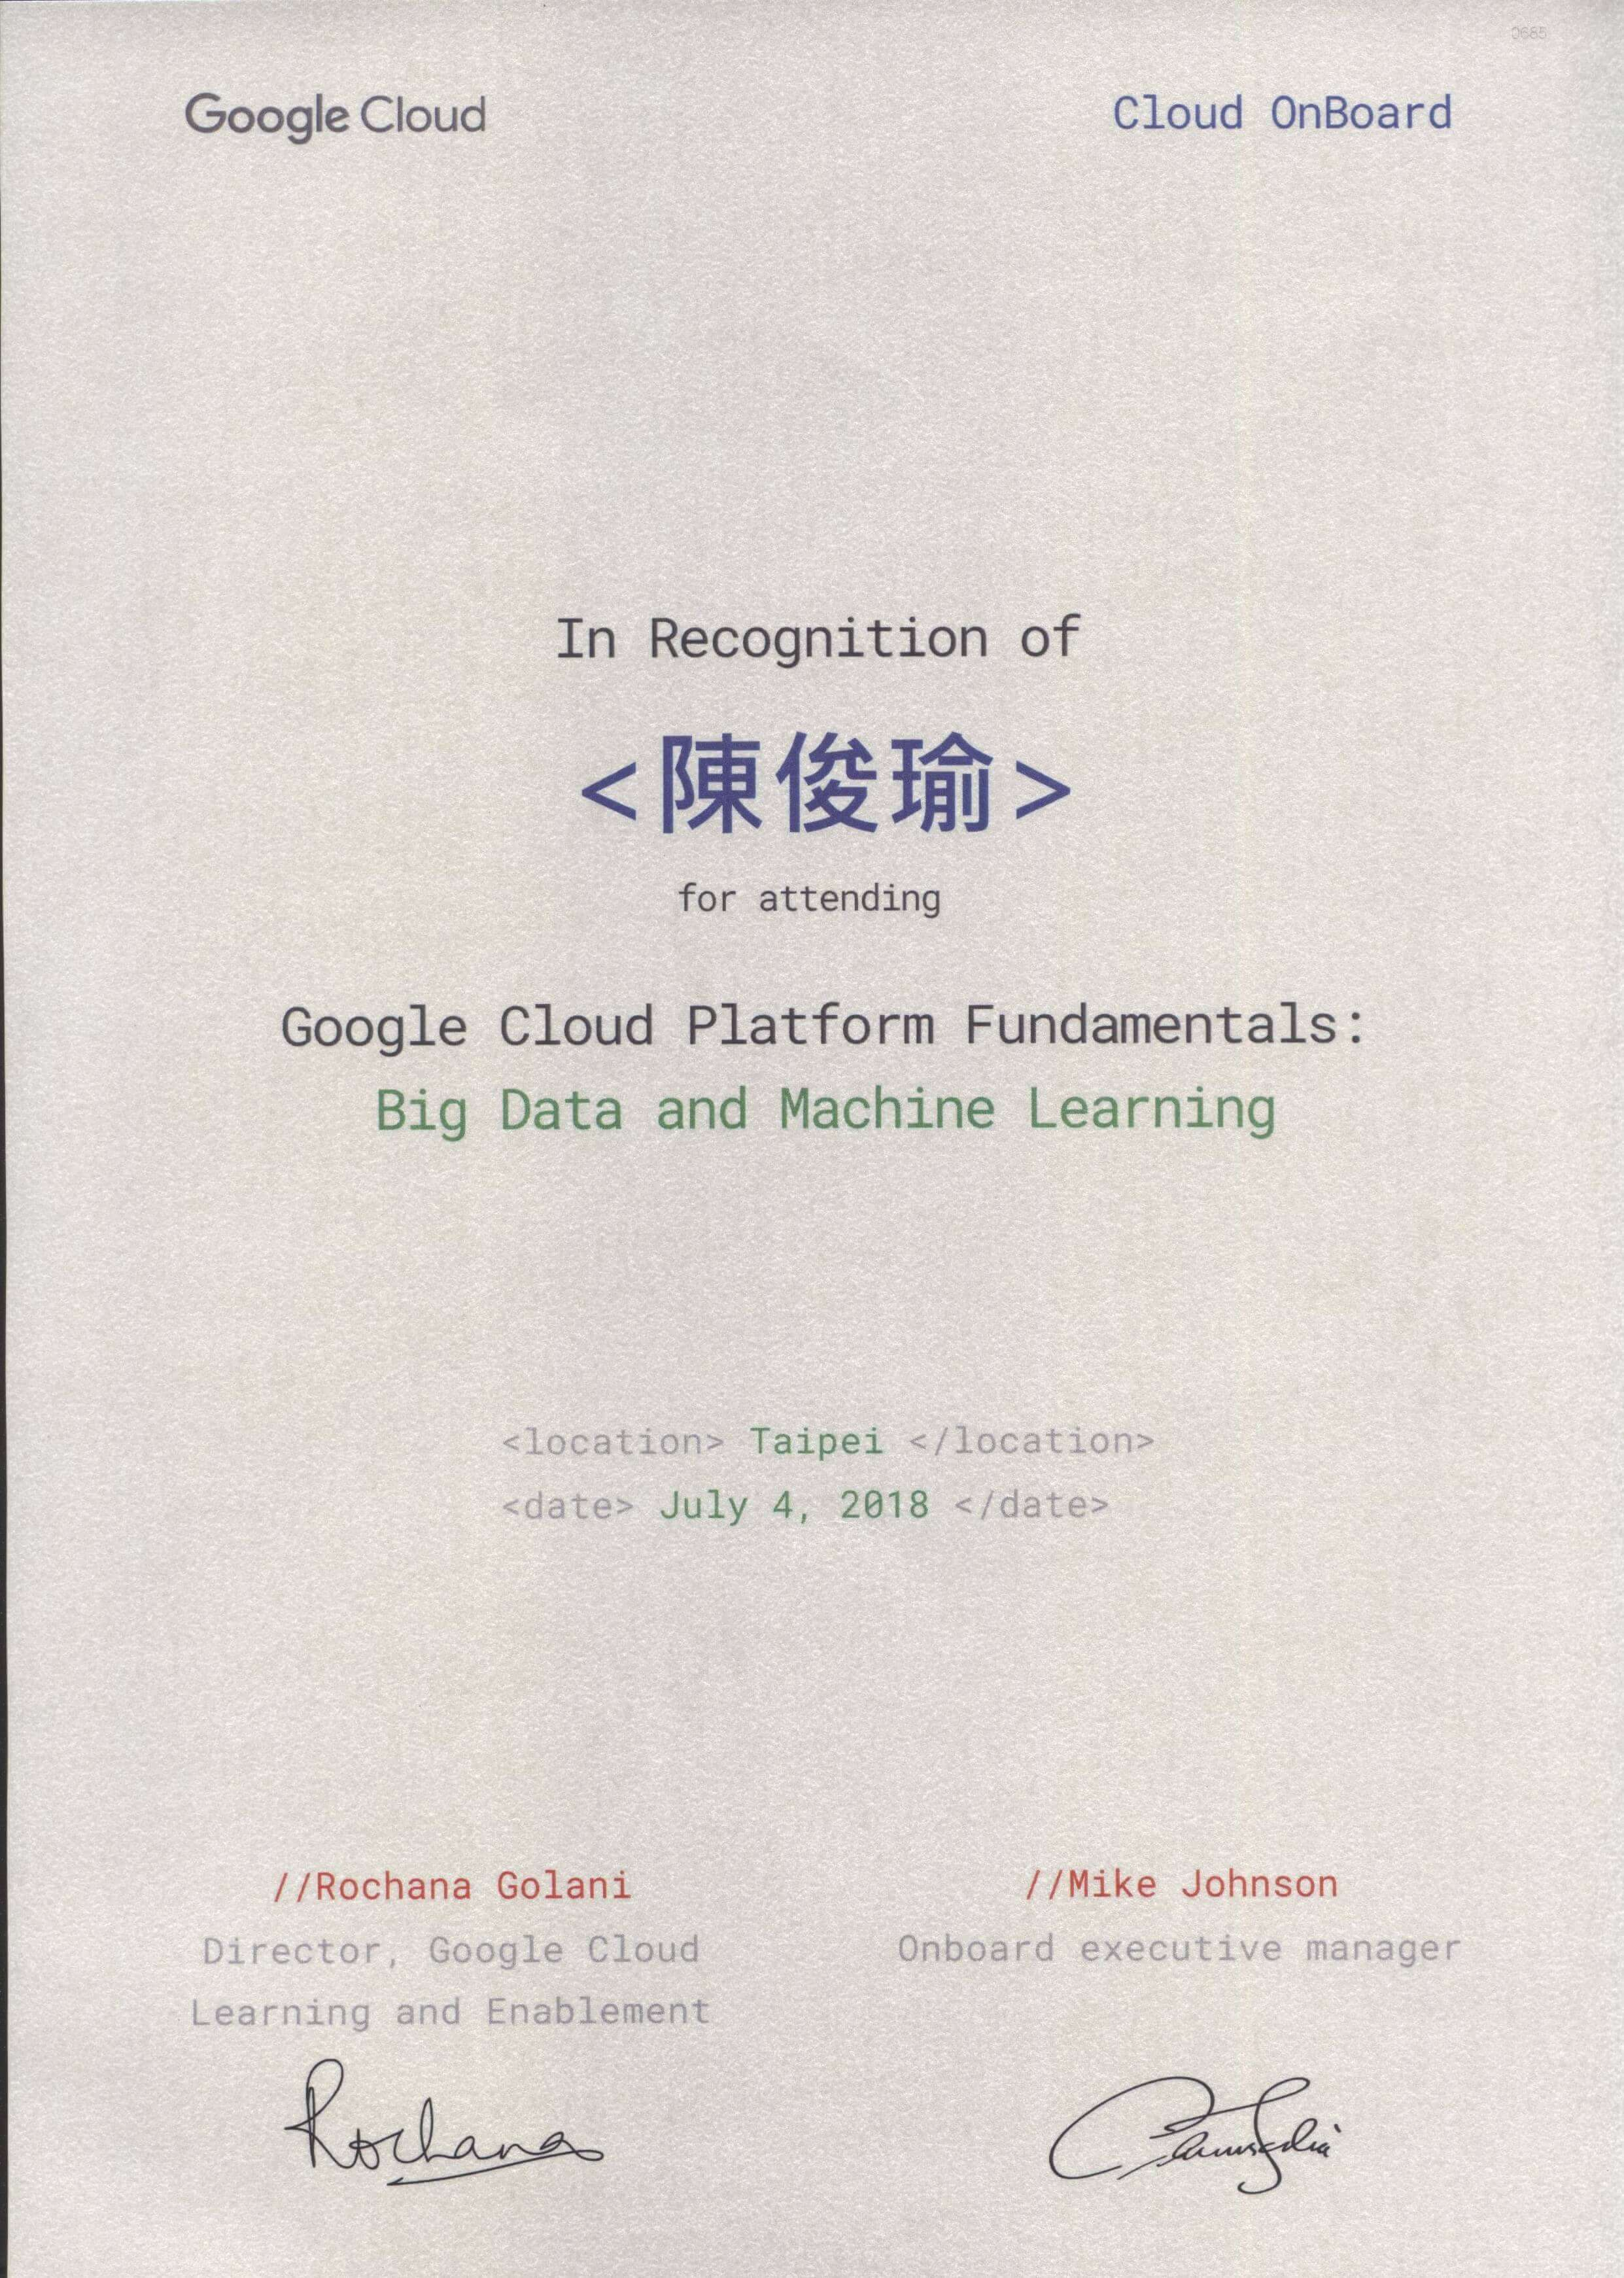
\includegraphics[width=0.3\textwidth]{images/Google Cloud OnBoard.jpg}
%     \caption{證書}
% \end{figure}

\subsection{大學}

\subsubsection*{2019}

\begin{itemize}
\tightlist
\item
  COSCUP 開源人年會
\item
  LASS 使用者與開發者大會
\end{itemize}

\subsubsection*{2020}

\begin{itemize}
\tightlist
\item
  COSCUP 開源人年會
\item
  SITCON 學生計算機年會
\end{itemize}

\subsubsection*{2021}

\begin{itemize}
\tightlist
\item
  COSCUP 開源人年會
\item
  SITCON 學生計算機年會
\end{itemize}
\newpage
\section{學生組織參與}

\begin{itemize}
\tightlist
\item
  學生活動中心:主要管理學校的活動場地,有活動時需要值班,需要為活動方控制場地設備,維持場地的清潔。平常各部門也會組織團建活動,在裡面認識了不少本科系以外的同學。
\item
  昇華工作室
  程序部:主要做一些網頁設計、開發工作,維護學校官方的小程序,也在裡面認識了一些寫程式很厲害的大佬。
\item
  網路服務隊:一個幫助校內師生維修電腦的學生組織,在裡面學習了硬體知識和裝電腦的經驗。我擅長處理系統問題,\textbf{Linux 問題一般由我來修},也會幫別人拆電腦清灰。
\end{itemize}
\begin{figure}[H]
    \centering
    \includegraphics[height=0.8\textwidth]{images/活動中心聘書.jpg}
    \caption{學生活動中心的助理聘書}
\end{figure}

\part{高中獎狀}

\section{專題網頁競賽佳作}

\begin{figure}[H]
    \centering
    \includegraphics[height=0.8\textwidth]{images/網頁比賽.jpg}
    \caption{專題網頁競賽佳作獎狀}
\end{figure}

\section{高一資訊能力競賽佳作}

\begin{figure}[H]
    \centering
    \includegraphics[height=0.8\textwidth]{images/高一資訊能力競賽佳作.jpg}
    \caption{高一資訊能力競賽佳作獎狀}
\end{figure}

\section{高三資訊能力競賽第三名}

\begin{figure}[H]
    \centering
    \includegraphics[height=0.8\textwidth]{images/高三資訊能力競賽.jpg}
    \caption{高三資訊能力競賽第三名獎狀}
\end{figure}

\section{高中科展 生活與應用科學組 優等}

\begin{figure}[H]
    \centering
    \includegraphics[height=0.8\textwidth]{images/科展.jpg}
    \caption{高中科展 生活與應用科學組 優等獎狀}
\end{figure}
\end{document}

